\documentclass[10.5pt,a4paper]{article}

\usepackage[top=0.75in,bottom=0.75in,left=0.85in,right=0.85in]{geometry}
\usepackage{times}
\usepackage{titlesec}
\usepackage{enumitem}
\usepackage{booktabs}
\usepackage{tabularx}
\usepackage{array}
\usepackage{hyperref}
\usepackage{parskip}
\usepackage{microtype}
\usepackage{tikz}
\usepackage{mdframed}
\usepackage{xcolor}
\usetikzlibrary{shapes.geometric, arrows.meta, positioning, fit, backgrounds}

\hypersetup{colorlinks=true, linkcolor=black, urlcolor=blue}

\titlespacing{\section}{0pt}{5pt}{2pt}
\titlespacing{\subsection}{0pt}{4pt}{1pt}
\titleformat{\section}{\normalfont\large\bfseries}{\thesection}{1em}{}
\titleformat{\subsection}{\normalfont\normalsize\bfseries}{\thesubsection}{1em}{}

\setlength{\parskip}{2.5pt}
\setlength{\parindent}{0pt}

\begin{document}

% ── Title ──────────────────────────────────────────────────────────────────────
\begin{center}
  {\LARGE \textbf{Building a Self-Updating Personal Knowledge Base with LLMs}}\\[5pt]
  {\large A Global Bread Encyclopedia Powered by Claude}\\[3pt]
  {\normalsize May 2026}
\end{center}

\hrule
\vspace{5pt}

% ── Links box ─────────────────────────────────────────────────────────────────
\begin{mdframed}[backgroundcolor=gray!8, linecolor=gray!40, linewidth=0.5pt,
                 innertopmargin=5pt, innerbottommargin=5pt,
                 innerleftmargin=8pt, innerrightmargin=8pt]
\small
\textbf{Live Demo:}~~\url{https://evelynlunlunding-sys.github.io/bread-knowledge-base/}\\
\textbf{Source Code:}~~\url{https://github.com/evelynlunlunding-sys/bread-knowledge-base}
\end{mdframed}

\vspace{3pt}

% ── Abstract ───────────────────────────────────────────────────────────────────
\textbf{Abstract.}
We present a self-updating personal knowledge base focused on global bread culture, implemented following the LLM-as-compiler workflow described by Karpathy. The system automatically ingests data from Wikipedia and web sources, uses Claude to synthesize raw content into structured Markdown entries organized by country and bread type, and exposes a CLI query interface and a publicly hosted browser-based frontend. A tiered auto-update scheduler refreshes individual entries monthly and discovers new categories annually. We compiled an initial corpus of 20 bread entries across 5 countries, demonstrating that LLMs can reliably maintain a structured, cross-linked knowledge wiki with minimal human intervention.

\vspace{3pt}
\hrule
\vspace{3pt}

% ── 1. Introduction ────────────────────────────────────────────────────────────
\section{Introduction}

The core insight behind LLM-powered knowledge bases is that language models excel not only at answering questions, but at \textit{organizing} knowledge---converting messy, heterogeneous raw data into clean, interlinked structured documents. Following Karpathy's workflow, we treat the LLM as a ``compiler'' that reads raw source documents from a \texttt{raw/} directory and incrementally builds a wiki of \texttt{.md} files, maintaining summaries, backlinks, and cross-references automatically.

We selected \textbf{global bread culture} as our knowledge domain. Bread is ideal for this exercise: it is well-documented across Wikipedia, recipe sites, and food blogs; it has a natural hierarchical structure (country $\rightarrow$ bread type $\rightarrow$ knowledge); and it has enough cross-cutting concepts (fermentation, leavening methods, regional variations) to make cross-linking genuinely useful. The resulting system covers 5 countries and 20 bread types, with each entry containing standardized sections for history, recipe, cultural context, and references.

% ── 2. System Architecture ─────────────────────────────────────────────────────
\section{System Architecture}

The system is organized into five decoupled modules:

\vspace{3pt}

\begin{center}
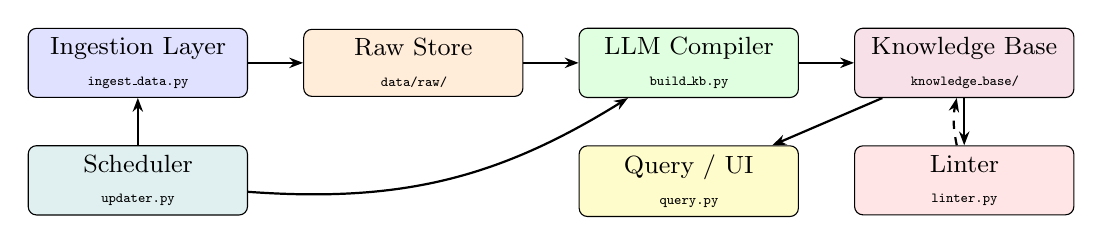
\begin{tikzpicture}[
  node distance=0.45cm and 0.7cm,
  box/.style={rectangle, rounded corners=3pt, draw=black, fill=gray!10,
              text width=2.55cm, align=center, minimum height=0.65cm, font=\small},
  arrow/.style={-{Stealth[length=5pt]}, thick},
]
\node[box, fill=blue!12] (ingest) {Ingestion Layer\\{\tiny \texttt{ingest\_data.py}}};
\node[box, fill=orange!15, right=of ingest] (raw) {Raw Store\\{\tiny \texttt{data/raw/}}};
\node[box, fill=green!12, right=of raw] (compiler) {LLM Compiler\\{\tiny \texttt{build\_kb.py}}};
\node[box, fill=purple!12, right=of compiler] (kb) {Knowledge Base\\{\tiny \texttt{knowledge\_base/}}};
\node[box, fill=red!10, below=0.6cm of kb] (linter) {Linter\\{\tiny \texttt{linter.py}}};
\node[box, fill=teal!12, below=0.6cm of ingest] (updater) {Scheduler\\{\tiny \texttt{updater.py}}};
\node[box, fill=yellow!20, below=0.6cm of compiler] (query) {Query / UI\\{\tiny \texttt{query.py}}};
\draw[arrow] (ingest) -- (raw);
\draw[arrow] (raw) -- (compiler);
\draw[arrow] (compiler) -- (kb);
\draw[arrow] (kb) -- (linter);
\draw[arrow] (kb) -- (query);
\draw[arrow] (updater) -- (ingest);
\draw[arrow] (updater) to[bend right=18] (compiler);
\draw[arrow, dashed] (linter) to[bend left=12] (kb);
\end{tikzpicture}
\end{center}

\vspace{3pt}

\begin{itemize}[leftmargin=*, itemsep=1.5pt]
  \item \textbf{Ingestion Layer} (\texttt{ingest\_data.py}): scrapes Wikipedia and public recipe sites using \texttt{requests} and \texttt{BeautifulSoup}, downloads images locally, and saves structured JSON to \texttt{data/raw/<country>/<bread>/}.
  \item \textbf{LLM Compiler} (\texttt{build\_knowledge\_base.py}): reads raw JSON, calls Claude to synthesize multiple sources into a single \texttt{.md} file, or \textit{merges} new sources into an existing entry without full rewrite.
  \item \textbf{Knowledge Base}: flat-file Markdown store at \texttt{knowledge\_base/<Country>/<bread>.md}, each with 9 required sections and YAML frontmatter. Fully Obsidian-compatible.
  \item \textbf{Auto-Updater} (\texttt{updater.py}): monthly bread refresh + yearly category discovery, with per-entry timestamps to skip recently-updated entries.
  \item \textbf{Query / UI}: a \texttt{click}-based CLI (\texttt{ask}, \texttt{compare}, \texttt{recipe}, \texttt{browse}, \texttt{search}) and a static HTML site hosted on GitHub Pages.
\end{itemize}

% ── 3. Implementation ──────────────────────────────────────────────────────────
\section{Implementation}

\subsection{LLM Compiler Design}

We use two Claude models with distinct roles. \textbf{Claude Opus 4.7} handles first-pass compilation where quality matters most: it receives all raw sources for a bread and produces the full structured Markdown document in a single call. \textbf{Claude Sonnet 4.6} handles incremental merges and interactive queries where speed and cost dominate. \textit{Prompt caching} (\texttt{cache\_control: ephemeral}) is applied to all system prompts, reducing token costs by $\sim$80\% on repeated calls within a session.

The compilation prompt enforces a strict 9-section schema enforced on every entry:

\vspace{2pt}
\begin{center}
\small\texttt{Overview $|$ Origin \& Country $|$ History $|$ Recipe $|$ Variations $|$ Cultural Context $|$ Images $|$ Related Breads $|$ References}
\end{center}
\vspace{2pt}

A cross-linking pass converts plain-text bread mentions into \texttt{[[wiki-link]]} syntax automatically after each build, enabling Obsidian-style graph navigation across the corpus.

\subsection{Data Quality: The Linter}

After each update cycle, \texttt{linter.py} runs two check layers: (1) \textit{rule-based} regex checks for missing required sections, broken image paths, and empty reference lists; (2) \textit{LLM-based} review where Claude checks each entry for factual inconsistencies, missing cultural context, and unlinked cross-references. Results are written to \texttt{lint\_report.md} and surfaced in the update log.

\subsection{Storage and Deployment}

Each Markdown file begins with YAML frontmatter (\texttt{title}, \texttt{country}, \texttt{tags}, \texttt{last\_updated}) followed by the nine content sections, stored as \texttt{knowledge\_base/<Country>/<bread>.md}. The static frontend is generated by \texttt{web\_ui.py} into \texttt{docs/} and deployed via GitHub Pages at the URL above---no server required.

% ── 4. Results ─────────────────────────────────────────────────────────────────
\section{Results and What Worked}

\begin{tabularx}{\linewidth}{lX}
\toprule
\textbf{Component} & \textbf{Outcome} \\
\midrule
Wikipedia ingestion & Reliable for all 20 breads; body text + image extraction \\
LLM synthesis & High-quality output: recipe tables, history timelines, cultural narratives \\
Cross-linking & Automatic; all entries link related breads via \texttt{[[wiki-links]]} \\
Query interface & \texttt{compare}, \texttt{recipe}, \texttt{browse} return accurate formatted answers \\
GitHub Pages & Zero-config public deployment; accessible without any local setup \\
Scheduler & Per-entry timestamps correctly prevent redundant re-ingestion \\
\bottomrule
\end{tabularx}

\vspace{3pt}

The LLM compiler's \textit{merge mode}---updating an existing entry without full rewrite---worked particularly well. It identified genuinely new facts from re-ingested sources and integrated them without duplicating content, behaving much like a human editor doing a targeted revision.

% ── 5. Limitations & Future Work ───────────────────────────────────────────────
\section{Limitations and Future Improvements}

\textbf{Limitations encountered during development:}
\begin{itemize}[leftmargin=*, itemsep=1pt]
  \item Major recipe sites (The Spruce Eats, AllRecipes) returned \texttt{402 Payment Required}, limiting secondary sources to Wikipedia only for most entries.
  \item Several LLM outputs were wrapped in a \texttt{```markdown} code fence, causing raw-text display in the web UI and requiring a post-processing cleanup pass and prompt refinement.
  \item Python 3.9 (Anaconda default) does not support the \texttt{X | Y} union-type syntax introduced in 3.10, requiring \texttt{from \_\_future\_\_ import annotations} across all modules.
\end{itemize}

\textbf{Planned future improvements:}
\begin{itemize}[leftmargin=*, itemsep=1pt]
  \item \textbf{RAG / vector search}: embed all entries with a text embedding model (e.g.\ \texttt{text-embedding-3-large}) and use FAISS or ChromaDB for semantic retrieval, enabling queries to scale beyond the context window.
  \item \textbf{Fine-tuning}: once the corpus reaches $\sim$500+ entries, fine-tune a smaller model to internalize the knowledge base in its weights rather than relying solely on in-context retrieval.
  \item \textbf{Image understanding}: use Claude's vision API to analyze bread images and auto-populate the Images section with descriptive captions (crumb structure, crust color, shape).
  \item \textbf{Multi-language support}: generate parallel entries in French, Italian, and German to capture region-specific baking terminology not well-represented in English sources.
  \item \textbf{Recommendation system}: build a bread-similarity graph from ingredient and technique overlap for ``users who like sourdough may also enjoy\ldots'' discovery.
  \item \textbf{Richer ingestion}: integrate Semantic Scholar for peer-reviewed food science papers and the YouTube Data API for video recipe transcript ingestion.
\end{itemize}

\vspace{5pt}
\hrule
\vspace{4pt}

{\small
\textbf{Deliverables summary:} 6 Python modules (1,500+ lines), 20 compiled knowledge base entries across 5 countries ($\sim$80,000 words of structured content), a tiered auto-update scheduler, an LLM-powered CLI query interface, a static web frontend deployed on GitHub Pages, and a data-quality linter. Source code and live demo links are provided above.
}

\end{document}
